\begin{frame}
\titlepage{}
\end{frame}

\section{Общая характеристика работы}

\begin{frame}
\frametitle{Проблема}
В приложениях реального времени существует потребность в симуляции огня
(рис.~\ref{fig:doomEternal}).

Требования и ограничения, предъявляемые к решению:
\begin{wrapfigure}{r}{0.5\textwidth}
	\centering
    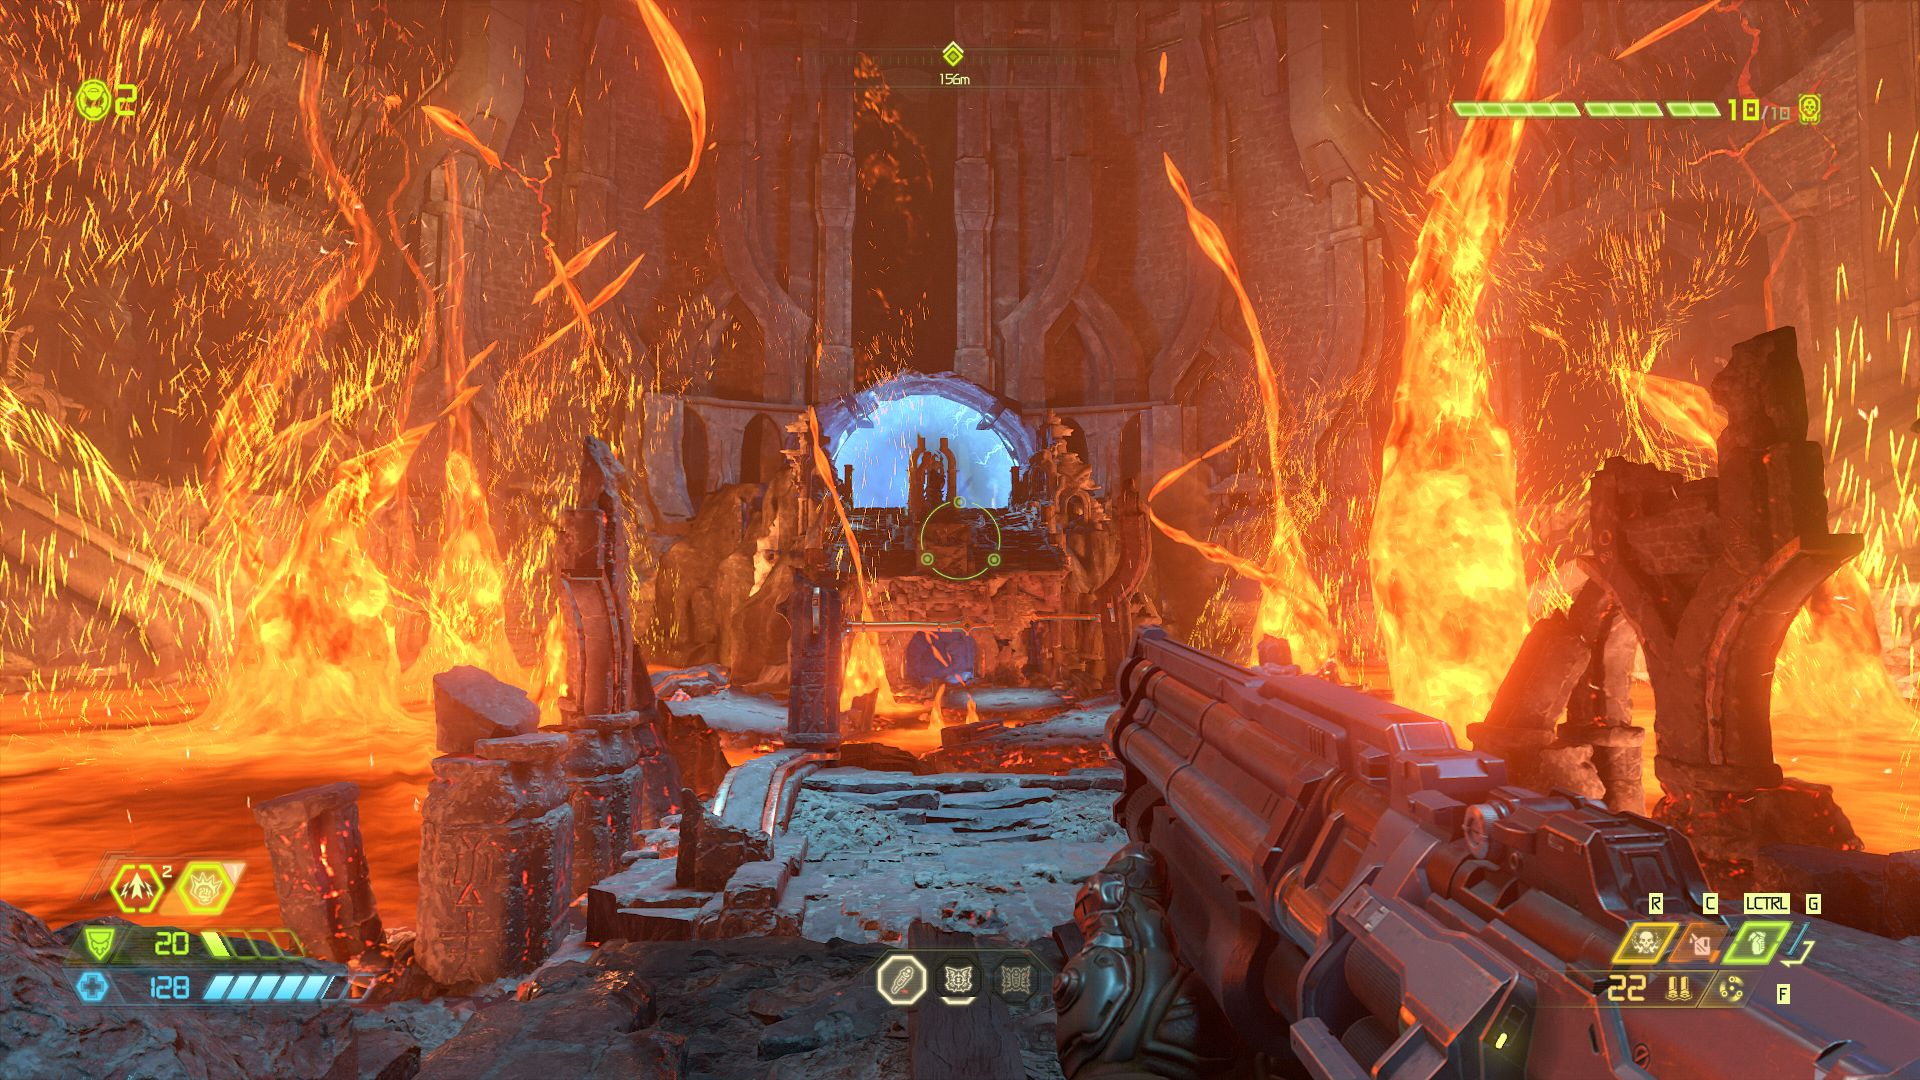
\includegraphics[width=0.5\textwidth]{DoomEternal}
    \caption{Кадр из игры Doom Eternal}%
    \label{fig:doomEternal}
\end{wrapfigure}
\begin{itemize}
    \item средняя частота кадров сцены --- 60 кадров /сек.;
    \item максимальная визуальная привлекательность;
    \item адаптивность под задачи художников.
\end{itemize}
\end{frame}

\section{Постановка задачи}
\begin{frame}
\frametitle{Цели и задачи исследования}
\textbf{Объектом исследования} является огонь в трехмерной графике как один из
элементов трехмерной сцены.

\textbf{Предметом исследования} является динамическая симуляция объемного огня в
режиме реального времени.

\textbf{Цель исследования} --- разработка системы динамической симуляции
трехмерного огня.

\textbf{Задачи исследования:}
\begin{enumerate}
	\item Обзор и анализ научных работ по современным алгоритмам анимации огня и
        трехмерному рендерингу.
	\item Анализ теории динамической симуляции огня.
	\item Реализация системы динамической симуляции.
\end{enumerate}
\end{frame}

\section{Анализ литературных источников}
\begin{frame}
\frametitle{Анализ методов симуляции огня}
В 2011 году Чжао Хуэй и его коллеги представили статью~\cite{survey}, в которой
авторы проанализировали большое количество методов симуляции огня и предложили
свою классификацию методов.

Результаты данного исследования можно увидеть в
таблице~\ref{table:algoAnalsysis}.
\begin{table}[htb]
    \caption{Сравнение производительности различных методов симуляции огня}
    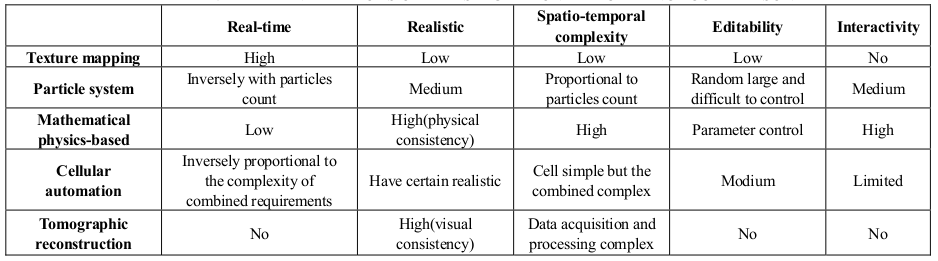
\includegraphics[width=\textwidth]{simulation_methods}%
    \label{table:algoAnalsysis}
\end{table}
\end{frame}

\section{Теория динамической симуляции огня}
\begin{frame}
\frametitle{Структура симуляции}
В общем случае задача симуляции огня может быть разбита на три
непересекающихся подзадачи~\cite{Perry94synthesizingflames}:
\begin{wrapfigure}{r}{0.5\textwidth}
	\centering
    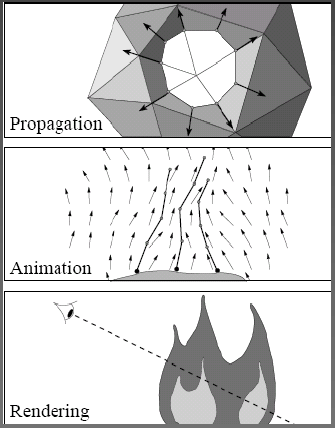
\includegraphics[width=0.27\textwidth]{simStages}
    \caption{Структура симуляции, предложенная в~\cite{realistic_sim}}%
    \label{fig:simStages}
\end{wrapfigure}
\begin{itemize}
	\item моделирование;
	\item анимация;
	\item визуализация.
\end{itemize}
Альтернативная схема была предложена Филиппом Боденом в
работе~\cite{realistic_sim} (рис.~\ref{fig:simStages}).
\end{frame}

\section{Техническое решение}
\begin{frame}
\frametitle{Идея решения}
В процессе анализа предыдущих работ по данной теме были выделены следующие идеи,
которые легли в основу технического решения:
\begin{enumerate}
    \item Визуальная эффектность симуляции важнее реалистичности.
    \item Физико-математические методы позволяют достичь высокой реалистичности
        анимации, однако требуют больших затрат ресурсов.
    \item Использование аналогий при анимации позволит существенно
        уменьшить количество расчетов по сравнению с численными методами.
\end{enumerate}
\end{frame}

\begin{frame}
\frametitle{Список использованных источников}
\sloppy\printbibliography[
    notcategory=AuthorSources,
    heading=none,
    resetnumbers,
]
\end{frame}

% \begin{frame}
% \frametitle{Outline}
% \tableofcontents
% \end{frame}
